\section{Scalogram interpretation}

The cwt is applied to all 28 ROI for each subject. The data contains the time series of pixel intensities for each of the 28 ROI for each recording of a subject.  
The output of the cwt is a scalorgram showing the time-frequency analysis content of the data. Frequencies of higher magnitude will show up with brighter colors, which can also be seen on the magnitude colorbar for comparison of the magnitude with related values.
The frequency of the scalograms varies from 2.7370 Hz to 0.0031 Hz. This means according to the literature, that bands of cardiac, respiratory, endothelial, myogenic and neurogenic is represented in the wavelet frequency span for the time frequency analysis. \cite{gayer2004, sagaidachnyi2014}

The scalogram in \figref{fig:scalogram_uncorr} is representing the cwt of the raw signal for region eight from subject three.

\begin{figure}[H]
	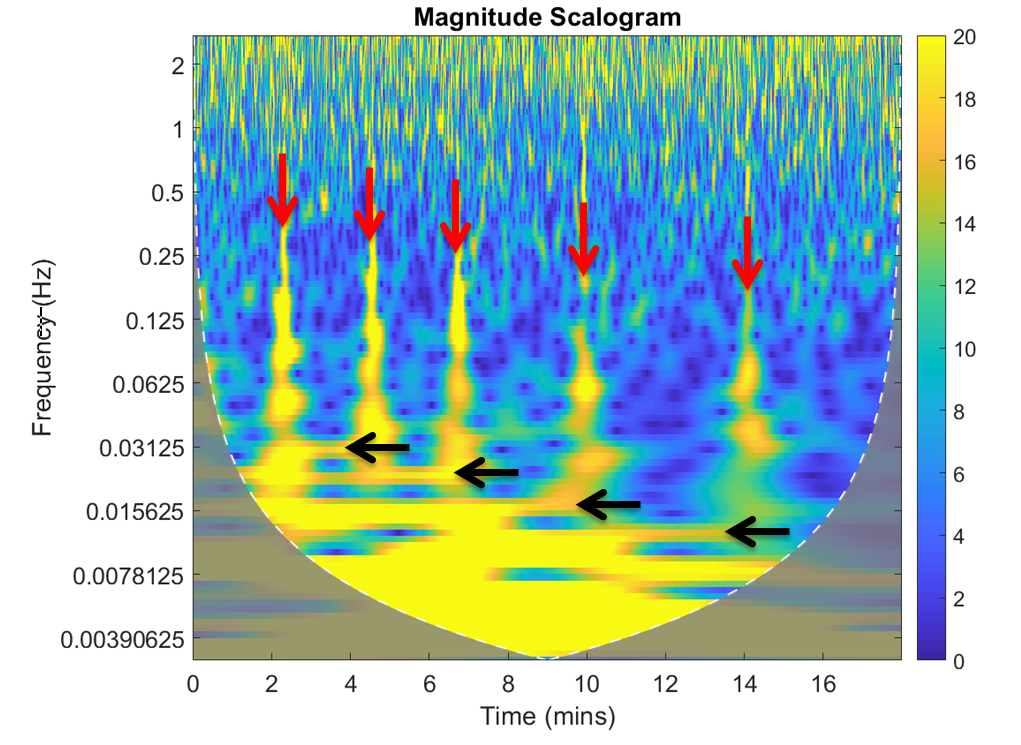
\includegraphics[width=0.7\textwidth]{figures/uncuffed_sub3_roi8_uncorr}
	\caption{Scalogram from the raw data from region eight in the uncuffed recording of subject 3.}
	\label{fig:scalogram_uncorr}
\end{figure}

Looking at the scalogram from the raw signal in \figref{fig:scalogram_uncorr} the jumps can easily be seen as the hight spikes which represents the jumps in the signal. Five jumps that are indicated with the red arrows, are present in the scalogram at time points around 2.5, 4.5, 6.5, 10 and 14 in the signal. The jumps in the same signal shown in the time domain shows jumps at the same time points. It is presumed that the corrected drift also is represented in the scalogram as low frequency content. Hereby different artifact components can be presumed to be included in the signal content. 

The artifact components of the raw signal can be sorted into three categories: 
\begin{itemize}
	\item Uniform white noise artifacts
    \item Drift artifacts between each interval
	\item Jumps artifacts
%	\item Generel drift in the signal
\end{itemize}

Uniform white noise artifacts is characterized by having the same magnitude in all frequencies. This artifact will therefore not affect the signal of interest, because it will have a flat power spectral density throughout the bandwidth of the frequencies, because the signals of the white noise are independent and evenly distributed \cite{hida2014}. 
The jumps in the signal is induces by the auto-adjustments from the camera described in \ref{sec:artifacts}. The drift artifacts can be seen in the magnitude under the jumps as different frequencies, this is because the drift is not uniform between intervals.
The artifact components is disturbing the signal to get a representative cwt of the signal of interest, which can be hidden by these artifacts. The artifacts is not constant for each recording, why the correction of the signal has been implemented shown in figure \figref{fig:scalogram_corr}.

\begin{figure}[H]
	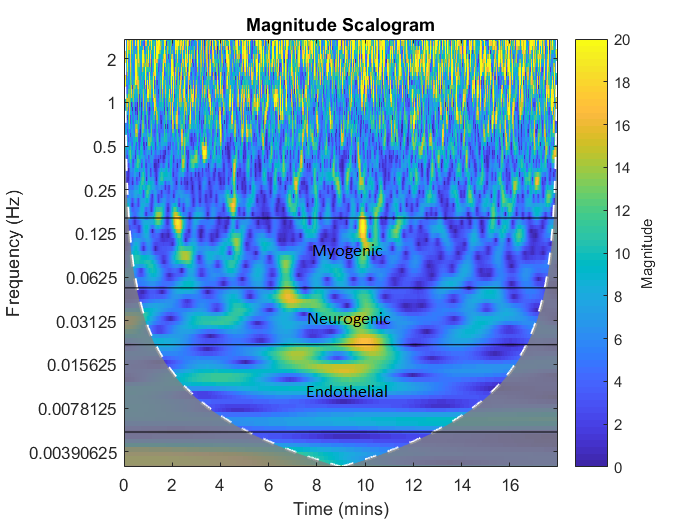
\includegraphics[width=0.7\textwidth]{figures/uncuffed_sub3_roi8_corr}
	\caption{Scalogram from the corrected data of region 8 in the uncuffed recording of subject 3, where a dampening of the spikes and  induced by the jumps has been achieved.}
	\label{fig:scalogram_corr}
\end{figure} 

After the correction of the signal, the energy  has been reduced at the areas induced from the jumps and the drift. The scalogram is left with less enery overall as seen in \figref{scalogram_corr}. %It can be discussed if the correction of the signal affects the signal of interest. 

The three frequency bands are shown with lines in the scalogram of \figref{scalogram_corr}.
To prepare the data for the statistical test, the averaged magnitude over the time period of each frequency band are first calculated be equation \ref{eq:W_avg}.
\begin{flalign}
W(n_{f})=\frac{1}{N} \sum_{n=1}^{N} W_n(n_{f})
\label{eq:W_avg}
\end{flalign}
Where N denotes the total number of elements in the frequenzy band, W is the magnitude of the wavelet, $n_{f}$ is the respective frame and n is the current element of the magnitude of the frequency band.

Then the mean of the average over the time period is calculated by equation \ref{eq:W_mean}
\begin{flalign}
	W_{mean}=\frac{1}{N_{f}} \sum_{n_f=1}^{N_{f}} W(n_{f})
	\label{eq:W_mean}
\end{flalign}
Where $W_{mean}$ denotes the mean value of the frequency band over the time period and $N_{f}$ is the total number of frames.
This gives a single value for the specific frequency band to be used in the statistical test for comparison between uncuffed and cuffed condition.